% Asset ID: AS1TrigonometricRatiosTIKZ-005
% Source: P1-Chp9 pp.17-18
% Related section: Ambiguous Case
% Purpose: Two possible triangles
\documentclass[tikz,border=8pt]{standalone}
\usepackage{amsmath}
\usetikzlibrary{angles,quotes,calc,arrows.meta}
\begin{document}
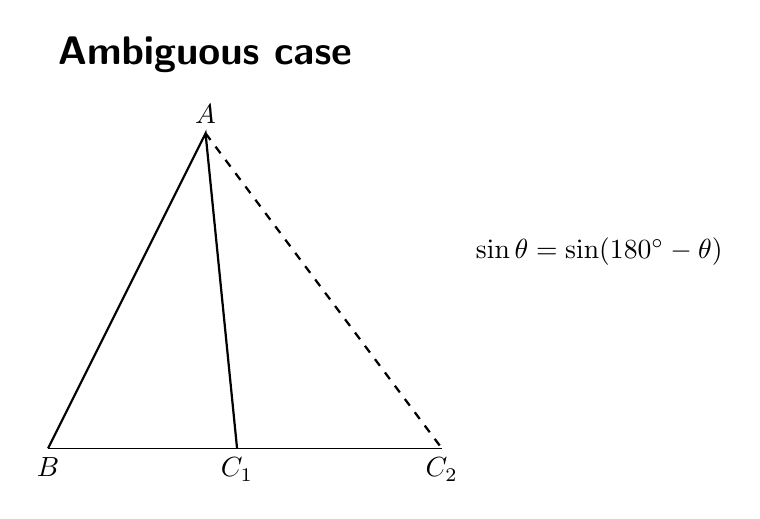
\begin{tikzpicture}[scale=1.0, every node/.style={font=\sffamily}]
\node[font=\sffamily\bfseries\Large, anchor=west] at (0,5) {Ambiguous case};
\coordinate (B) at (0,0);\coordinate (A) at (2,4);\coordinate (C1) at (2.4,0);\coordinate (C2) at (5,0);\draw[thick] (B)--(A)--(C1);\draw[thick,dashed] (A)--(C2);\draw (B)--(C2);\node[above] at (A) {$A$};\node[below] at (B) {$B$};\node[below] at (C1) {$C_1$};\node[below] at (C2) {$C_2$};\node at (7,2.5) {$\sin\theta=\sin(180^\circ-\theta)$};
\end{tikzpicture}
\end{document}
